\subsection{Singular Value Decomposition (SVD) ($A = U \Sigma V^\top$)}


\begin{figure}[H]
    \centering
    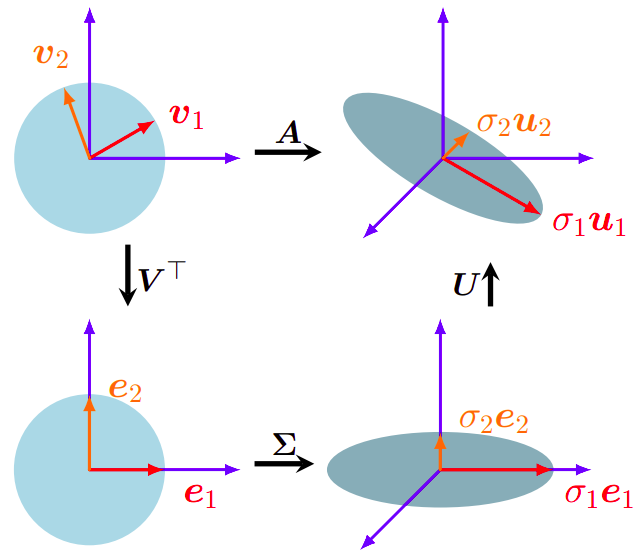
\includegraphics[
        width=\linewidth,
        height=5cm,
        keepaspectratio,
    ]{images/maths-for-ml/singular-value-decomposition.png}
    \caption*{
        Intuition behind the SVD of a matrix $\bm{A} \in \mathbb{R}^{3\times 2}$ as sequential transformations.
        \\
        \textbf{Top-left to bottom-left}: $\bm{V}^\top$ performs a basis change in $\mathbb{R}^2$.
        \\
        \textbf{Bottom-left to bottom-right}: $\Sigma$ scales and maps from $\mathbb{R}^2$ to $\mathbb{R}^3$ . The ellipse in the bottom-right lives in $\mathbb{R}^3$. The third dimension is orthogonal to the surface of the elliptical disk.
        \\
        \textbf{Bottom-right to top-right}: $\bm{U}$ performs a basis change within $\mathbb{R}^3$.
    }
\end{figure}


\begin{enumerate}
    \item The singular value decomposition (SVD) of a matrix is a central matrix decomposition method in linear algebra.
    \hfill \cite{mfml/book/mml/Deisenroth-Faisal-Ong}

    \item It has been referred to as the “fundamental theorem of linear algebra” because it can be applied to \textbf{all matrices}, not only to square matrices, and it \textbf{always exists}.
    \hfill \cite{mfml/book/mml/Deisenroth-Faisal-Ong}

    \item the SVD of a matrix $\bm{A}$, which represents a linear mapping $\Phi : V \to W$, quantifies the change between the underlying geometry of these two vector spaces.
    \hfill \cite{mfml/book/mml/Deisenroth-Faisal-Ong}

    \item 
    \begin{theorem}[SVD Theorem]
        Let $\bm{A} \in \mathbb{R}^{m\times n}$ be a rectangular matrix of rank $r \in [0,\ \min(m, n)]$. 
        The SVD of $\bm{A}$ is a decomposition of the form 
        $
            \underset{\displaystyle m\times n}{\underbrace{\bm{A}}} = 
            \underset{\displaystyle m\times m}{\underbrace{\bm{U}}}\ 
            \underset{\displaystyle m\times n}{\underbrace{\bm{\Sigma}}}\ 
            \underset{\displaystyle n\times n}{\underbrace{\bm{V}^\top}}
        $ 
        with an orthogonal matrix $\bm{U} \in \mathbb{R}^{m\times m}$ with column vectors $\bm{u}_i$ , $i = 1, \cdots , m$, and an orthogonal matrix $\bm{V} \in \mathbb{R}^{n\times n}$ with column vectors $\bm{v}_j$ , $j = 1, \cdots , n$.
        Moreover, $\bm{\Sigma}$ is an $m \times n$ matrix with $\Sigma_{ii} = \sigma_i \geq 0$ and $\Sigma_{ij} = 0, i \neq j$.
        \hfill \cite{mfml/book/mml/Deisenroth-Faisal-Ong}
    \end{theorem}
\end{enumerate}










